%%%%%%%%% BODY TEXT


\section{Overview}
This supplementary document provides more discussions and experimental details. 
In Sec.~\ref{sec:more_discussion}, we discuss in detail the differences between our method and state-of-the-art approaches. 
Details about network architecture are presented in Sec.~\ref{sec:imp_details}. 
In Sec.~\ref{sec:exp_details} we present more details about how we collect the data and how we conduct the experiments. 
We conduct additional experiments in Sec.~\ref{sec:more_exp} to further evaluate our method design. 
Finally, we discuss the limitations and potential future work in Sec.~\ref{sec:limitation}. 
Please refer to the supplementary video for more visualizations. 

\section{More Discussion}
\label{sec:more_discussion}
% \subsection{Discussion on SOTA Methods}
Our method aims at creating a controllable 3D human character from RGB videos without pre-scanning a subject-specitic template. 
To better motivate our method and differentiate from existing approaches, we list the most related works below and discuss their limitations as well as our solution in this section. 

\textbf{Neural Body}~\cite{peng2021neuralbody} attaches learnable latent codes to the vertices of SMPL model, and employs sparse 3D convolutions to diffuse the latent codes into a radiance field in the 3D space. This scheme shows impressive performance on novel view synthesis for human performance. However, it struggles with new pose syntheses, as shown in \cite{peng2021animatable_nerf}. The main reason for this limitation is that 3D convolution is not equivalent to spatial changes of the structured latent code. In our method, we avoid the need for 3D convolutions and construct the radiance field by combining a set of localized ones, thus easily enable avatar animation by design.
% If we assume there is no overlap between any two local radiance fields, then our representation based on localized radiance fields is equivalent to spatial changes in nature, thus can easily enable avatar animation.

\textbf{Animatable NeRF}~\cite{peng2021animatable_nerf} factorizes a deforming human body into a canonical radiance field and per-frame deformation fields that establish correspondences between the observations and the canonical space. 
The deformation field is generated through diffusing the input skeleton motion into the 3D space based on the learnable blending weights. 
Thanks to the explicit disentanglement of shape and motion, Animatable NeRF~\cite{peng2021animatable_nerf} is able to synthesize images for unseen poses. 
However, the motion representation is too simple to model the complex non-rigid deformations of clothes, which results into unrealistic, static texture and even severe artifacts when applying this method on loose clothes. In contrast, our method explicitly takes into account the non-rigid cloth deformation via coarse-to-fine decomposition, and demonstrates plausible animation results for human characters wearing dresses. 


\textbf{Neural Actor}~\cite{neural_actors} shares a similar scheme with Animatable NeRF~\cite{peng2021animatable_nerf}: it also learns a neural radiance field in a canonical body pose, and use LBS to warp the canonical radiance field to represent the moving subject. Its main innovations are two fold: 1) Neural Actor learns pose-dependent non-rigid deformation that cannot be captured by standard skinning using a residual function, and 2) Neural Actor encodes appearance features on the 2D texture maps of the SMPL model to better capture dynamic details. Although this scheme shows impressive results in modeling the pose-dependent appearance details like the cloth wrinkles, it only works well for clothing that is topologically similar to the body. Besides, Neural Actor~\cite{neural_actors} requires multi-view input in order to obtain a complete texture map for network training. 
Note that we also use SMPL model in our approach; but we do not explicitly depend on the SMPL topology for shape and appearance representation. Therefore, our method is more general than Neural Actor~\cite{neural_actors} in terms of the cloth topology, and can work with partial input such as a monocular video. 


\textbf{DDC}~\cite{habermann2021realtimeDDC} is another state-of-the-art method for building animatable avatars. It demonstrates impressive results for loose clothes and even achieves real-time rendering performance. However, DDC requires a pre-scanned template model of the actor; that is why we do not compare with it since person-specific templates are not available in our experiment setting. In contrast, our method can model the dynamic shape and appearance of general garments without any pre-scanning efforts.


% As mentioned in Line 031/052/175 of the main paper, our work focuses on learning animatable characters \emph{without} person-specific templates. In this specific topic, [47,29] are the state-of-the-arts among existing works and yet not method has demonstrated results for loose clothes. 
% [18] can handle loose clothes but it \emph{requires a pre-scanned template model} of the actor; that is why we did not compare with [18] since person-specific templates are not available in our experiment setting. 
% In contrast, our method can model the dynamic shape and appearance of general garments without pre-scanning efforts.
% We agree that [18] is the state-of-the-art method for building avatars in loose clothes if pre-scanned templates are given. 
% We will refine the discussion of [18], correct the description in Line 47, clarify our problem setup and compare with [18] in the revision. 


Some methods like \textbf{TNR}~\cite{Shysheya2019TNR} and \textbf{ANR}~\cite{raj2020anr} learn animatable avatars in 2D domain. They typically define appearance features (RGB color values or high-dimensional features) on the UV map of a body template, and exploit a 2D convolutional network to obtain the final color image. These methods not only suffer from the same limitation as \cite{peng2021animatable_nerf,neural_actors}, but also fail to guarantee view consistency when rendering free-viewpoint images. Our method focuses more on creating a \textbf{3D} model, thereby significantly departing from this line of works. 




\textbf{MVP}~\cite{Lombardi2021MVP} also proposes to use local volumetric representation for deformable surface rendering. However, our work is essentially different from MVP:
1) MVP requires an estimate of scene geometry to construct the volumetric primitives, while our method works without knowing scene geometry; 
2) MVP assumes accurate tracking of scene geometry over time, while our method is carefully designed to directly learn the motion hierarchy from data; 
3) MVP only handles head movements and facial expressions, while our method can deal with challenging body motions and cloth deformations;  
4) MVP mainly focuses on efficient rendering of training frames, while our method supports novel pose generation with explicit pose control. 


% \subsection{Discussion on Method Design}
% \textbf{Why not using canonical NeRF?}
% A core difference between our method and existing ones (\textit{e.g.},  \cite{neural_actors,peng2021animatable_nerf}) is that our method does not explicitly define a canonical field and consequently avoids the need for ``backward skinning". 
% The reason behind this design is the ambiguity of backward skinning: when two body parts are in close proximity to each other, it is difficult to determine the canonical positions for the points around those body parts. In contrast, our scheme computes the radiance of any point in the posed space, thus resolving the ambiguity issue. 

% \textbf{Why time stamp?}







\section{Implementation Details}
\label{sec:imp_details}
\subsection{Architecture Details}

\begin{figure}
    \centering
    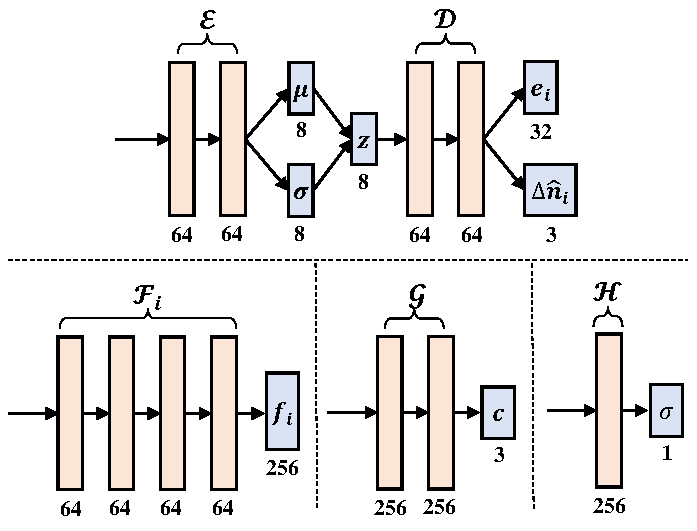
\includegraphics[width=1.0\linewidth]{arch_details}
    \caption{\textbf{Architecture of our network.} Each orange rectangle represents a fully-connected layer followed by ReLU activation, and the numbers of output channels are labeled underneath. }
    \label{fig:arch_details}
\end{figure}



We illustrate the network architecture in Fig.~\ref{fig:arch_details}. Note that before feeding the coordinates, view directions and time stamps into the MLP, we augment them using sinusoidal encoding, which is defined as: 
\begin{equation}
    \gamma (\bm{\mathrm{x}}) = \left(\bm{\mathrm{x}}, \sin(\bm{\mathrm{x}}), \cos(\bm{\mathrm{x}}), ..., \sin(2^{m-1}\bm{\mathrm{x}}), \cos(2^{m-1}\bm{\mathrm{x}}) \right). \nonumber
\end{equation}
The value of $m$ is 6 for coordinates, 4 for view directions and 12 for time stamps. We normalize the time stamp before sinusoidal encoding, \textit{e.g.}, the time stamp for $t$-th frame is normalized to $t/T$, where $T$ is the total number of frames. 

Note that the vanilla NeRF adopts a hierarchical sampling strategy and  simultaneously optimizes two networks (one ``coarse" and one ``fine"), while we only train one network with uniform sampling for fair comparison against baseline methods. 

\subsection{Network Acceleration}
Naively implementing our network will lead to heavy computational complexity, as one needs to query every local network for all point samples. 
% The number of network queries is $N\times S$, where $N$ and $S$ is the number of the nodes and point samples, respectively.
To reduce network queries and accelerate program execution, we exploit the fact that for any point in the posed space, only a small portion of nodes have an influence on its color and density value. This is because the influence range of the nodes is truncated, as mathematically defined in Eqn. 6.
Based on this observation, we implement custom CUDA kernels for acceleration purpose. 
To be more specific, let $S$ denote the number of point samples and $N$ the number of nodes (which is also the number of local MLPs). In the naive implementation, the points are first transformed into the local coordinate systems of the nodes, which results into a tensor of size $N\times S \times 3$ being fed into the network. In our optimized implementation, we first calculate the number of necessary point queries for each local MLP (indexed by $i$), which is denoted as $S_i$. 
Then we construct an empty tensor of size $N\times S' \times 3$, where $S' = \max\{S_1, S_2, ..., S_N\}$. By investigating the values of blending weights, we pick the valid elements in the original tensor and rearrange them into the new one, which is finally fed into the network. 
With our optimized implementation, the memory consumption decreases about 85\%, and the running time decreases by a factor of 4. 




\begin{table}
    \footnotesize
    \centering
    \caption{Hyperparameters for network training and evaluation. }
    \begin{tabular}{lc}
    \toprule
       Parameter Name & Value \\
    \midrule
    %   $\delta_s$ in $clamp(\cdot)$ & $0.1$ \\
       $N$ (Number of Nodes)                        & $128$ \\
       $\sigma$ (In Eqn. 6)                         & $0.05$ \\
       $\epsilon$ (In Eqn. 6)                       & $0.001$ \\
       $\lambda_{rec}$ (In Eqn. 11)                  & $1.0$ \\
       $\lambda_{trans}$ (In Eqn. 11)                & $0.02$ \\
       $\lambda_{ebd}$ (In Eqn. 11)                  & $0.1$ \\
       $\lambda_{KL}$ (In Eqn. 11)                   & $1\times 10^{-5}$ \\
    %   Fourier Frequency Number of Time Stamp           & $12$ \\ 
    %   Fourier Frequency Number of Coordinate           & $6$ \\ 
    %   Fourier Frequency Number of View Direction       & $4$ \\ 
       Dimension of $\bm{e}_i$ (In Eqn. 5)          & $32$  \\
       Dimension of $\bm{z}_i$ (In Eqn. 9)          & $8$  \\
       Number of Ray Samples Per Batch              & $2048$ \\
       Number of Point Samples Per Ray              & $64$ \\
       Batch Size                                   & $4$ \\
    %   Number of Iterations                         & $500,000$ \\
       Learning Rate                                & $5\times 10^{-4}$  \\
       Adam $\beta_1$                               & $0.9$ \\
       Adam $\beta_2$                               & $0.999$ \\
    \bottomrule
    \end{tabular}
    \label{tab:training_details}
\end{table}



\section{Experimental Details}
\label{sec:exp_details}
\subsection{Dataset}
In our experiments, we mainly use the following dataset: 
\begin{itemize}[leftmargin=*]
\setlength{\itemsep}{0pt}
% \setlength{\parsep}{0pt}
% \setlength{\parskip}{0pt}
\vspace{-0.2cm}
    \item Dataset from \cite{habermann2021realtimeDDC}. We use two dress sequences (``Ling" and ``FranziBlue") in this dataset. Each sequence contains about 20000 training frames captured using 100 cameras, but we manually select 20 views among them for computational efficiency. 
    \item Dataset from \cite{habermann2020deepcap}. We use one sweater sequence (``Lan") in this dataset, which is captured from 11 cameras and contains about 30000 training frames.   
    \item ZJU-MoCap dataset~\cite{peng2021neuralbody}. We mainly conduct experiments on two sequences (``CoreView387" and ``CoreView392"). Each sequence contains about 300 training frames captured from 23 view points, but we only use 4 view points among them for fair comparison against Neural Body~\cite{peng2021neuralbody}.  
    \item Multi-view dataset collected by ourselves. We built up a multi-view system that consists of 24 uniformly distributed cameras. Our system can capture synchronized videos at 30Hz with a resolution of 1024$\times$1024. We collect data for three subjects and the frame numbers of videos range from 2500 to 5000. 
\vspace{-0.2cm}
\end{itemize}

We use \cite{lightcap2021} to register SMPL(-X) model to the video frames, and use BackgroundMattingV2~\cite{BGMv2} for foreground segmentation. 

\subsection{Training Details}

We use PyTorch to implement our networks. The hyperparameters needed for network implementation and training are reported in Tab.~\ref{tab:training_details}. Note that during network training, the learning rate decays exponentially every 20k iterations. The number of iterations is set to 100k for People Snapshot dataset~\cite{alldieck2018videoavatar}, 300k for ZJU-MoCap dataset~\cite{peng2021neuralbody} and 500k for other multi-view sequences. 
For baseline methods, we use the author-provided code and run all the experiments using the default training settings.


\subsection{Metrics}
As described in the paper, we use two standard metrics, peak signal-to-noise ratio (PSNR) and structural similarity index (SSIM), for quantitative evaluation. To reduce the influence of background pixels, all the scores are calculated from the images cropped with a 2D bounding box which is estimated from the projection of SMPL model. More details are described in \href{https://github.com/zju3dv/neuralbody/blob/master/supplementary_material.md}{this link}. 


% For all baseline methods in comparison, we use their open-source code but replace their training/testing splits with ours for fair comparison. 
% All baseline methods and ours share the same training dataset and training configurations (e.g., learning rate, epoch number, optimizer settings, etc.), except that the batch size is manually adjusted to maximize GPU utilization. %Note that the epoch number is sufficient for all networks to converge. 
% All networks are trained on a single NVIDIA GeForce 2080 TI GPU. 


% \textbf{Discussion on the per-frame latent embedding in Neural Body} One may think that the poor generalization capability of Neural Body is because it uses per-frame latent embeddings ($\ell_i$ in \cite{}) to encode temporally varying details, and the latent embeddings for test poses are unknown. However, in our initial experiments, we observed that the latent embeddings have little influence on the rendering results: we replaced the latent embeddings in the pre-trained models (provided by the authors) with zero vectors, and found that the rendered images are almost identical with the images rendered using pre-trained latent embeddings (see Fig.\ref{}). Therefore, we conclude that the latent embeddings in Neural Body are actually unnecessary, and can be dropped in our experiments. 



\section{More Experiments}
\label{sec:more_exp}

\begin{table}
    \newcommand{\tabincell}[2]{\begin{tabular}{@{}#1@{}}#2\end{tabular}}
    \centering
    \scriptsize
    \caption{\textbf{Quantitative evaluation of the node-related variables.} We generate the images for training poses under different settings and report the averaged PSNR scores of all frames. }
    \label{tab:quant_node_effect}
    \scriptsize
    \begin{tabular}{lccc}
        \toprule
        Setting& w/o $\{\Delta\bm{n}_i^{(t)}\}$ or $\{\bm{e}_i^{(t)}\}$ & w/o $\{\bm{e}_i^{(t)}\}$ & Full  \\
        \midrule
        \tabincell{l}{Corresponding\\figure} & Fig.~3 (b) & Fig.~3 (c) & Fig.~3 (d)  \\
        \midrule
        PSNR & 17.52 & 20.47 & 21.48 \\ 
        \bottomrule
    \end{tabular}
\end{table}


\begin{table}
    \centering
    \scriptsize
    \caption{\textbf{Quantitative evaluation of our cVAE design.} We replace the cVAE with a determinstic regression network and report the reconstruction accuracy (PSNR) of training frames. }
    \label{tab:quant_cvae}
    \scriptsize
    \begin{tabular}{lcc}
        \toprule
        Setting& Deterministic & Ours  \\
        \midrule
        Corresponding figure & Fig.~9 (b,e) & Fig.~9 (c,f)  \\
        \midrule
        PSNR & 25.34 & 25.62 \\ 
        \bottomrule
    \end{tabular}
\end{table}


\noindent\textbf{Quantitative ablation of node-related variables.} We conduct a qualitative ablation study on the effects of the node-related variables in Fig.~3 in the main paper. In Tab.~\ref{tab:quant_node_effect} we report the corresponding quantitative results across all frames to further evaluate the impact of the node-related variables. 


\noindent\textbf{Quantitative ablation of our cVAE design.} Similarly, we report the corresponding quantitative results across all frames in Tab.~\ref{tab:quant_cvae} to further evaluate our cVAE design. The numeric results further prove that our cVAE design is critical for better reconstructing the realistic details in the training frames, which is consistent with our conclusion in the main paper. 


\begin{wrapfigure}{r}{0.35\linewidth}
\vspace{-2mm}
\hspace{-5mm}
% \centering
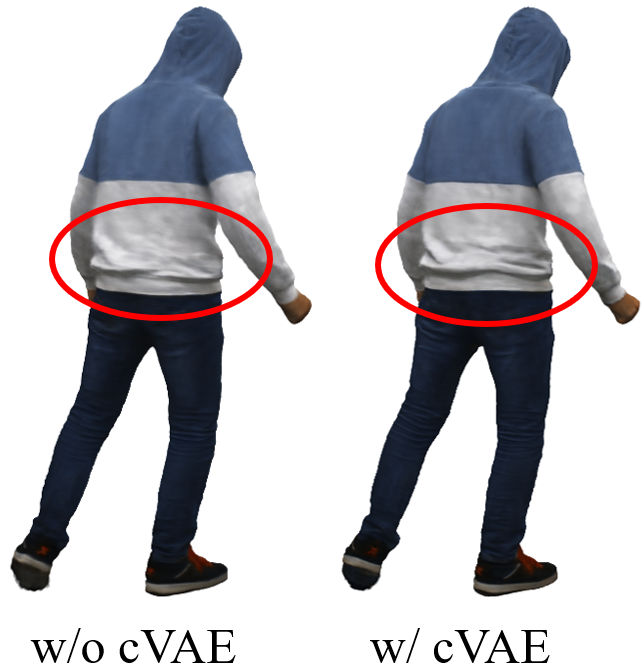
\includegraphics[width=1.01\linewidth]{eval_vae_test.png}
%   \caption{}
% \vspace{-3mm}
\end{wrapfigure}
\noindent\textbf{cVAE ablation with novel poses.} 
In Fig.~9 we mainly conduct the cVAE ablation study on training frames. 
In the right inset figure we conduct an identical experiment using novel poses from a testing sequence. The results also show that our cVAE design is benefitial for learning sharper wrinkle details. 



\begin{figure}
    \centering
    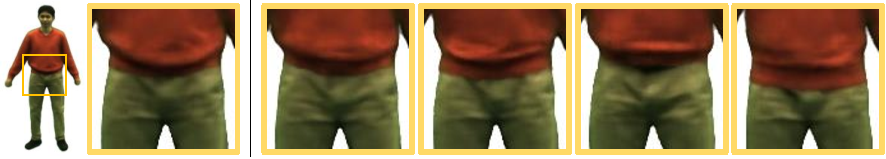
\includegraphics[width=1.0\linewidth]{random_z_small}
    \caption{\textbf{Impact of the latent $\bm{z}_i$.} We show the testing results when the same pose are given but $\bm{z}_i$ is set to zero (leftmost) or assigned with random Gaussian noises (right). }
    \label{fig:latent_z}
\end{figure}

\noindent\textbf{Impact of the latent $\bm{z}_i$.} As we mentioned in Sec.~4.1, we set $\bm{z}_i$ to zeros when synthesizing images of novel poses. In fact, latent $\bm{z}_i$ does not have to be zeros and can be modified in accordance of applications. In Fig.~\ref{fig:latent_z}, we show that modifying the latent $\bm{z}_i$ will lead to different wrinkle patterns. This feature can be further explored to generate multiple plausible animation sequences, and we leave it as future work. 





% \begin{figure}[h]
%   \begin{center}
%     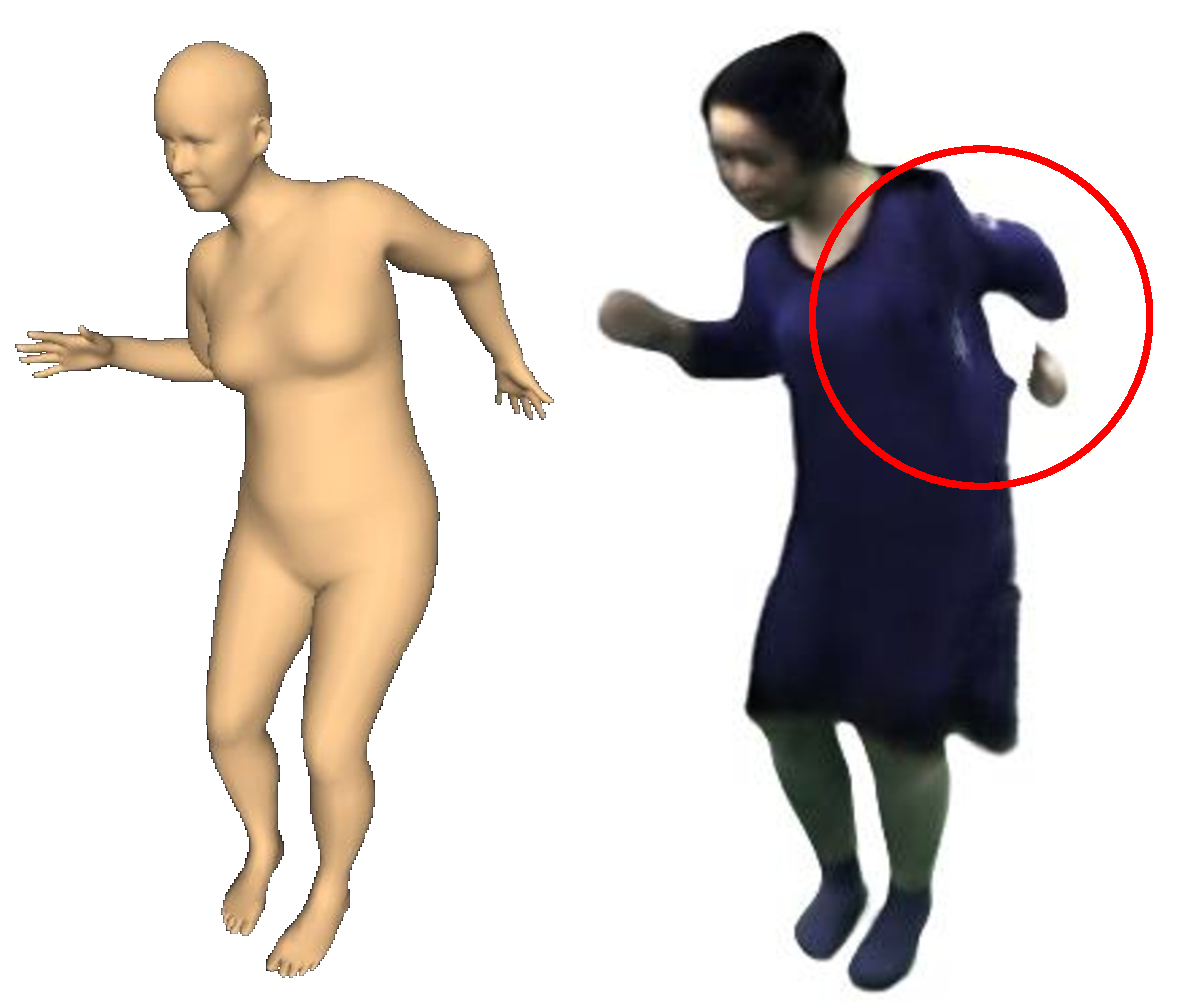
\includegraphics[width=0.5\linewidth]{failure}
%   \end{center}
%   \caption{Failure cases of our method.}
%   \label{fig:failure}
% \end{figure}



\section{Limitation and Future Work}
\label{sec:limitation}

\begin{wrapfigure}{r}{0.4\linewidth}
\vspace{-2mm}
\hspace{-5mm}
% \centering
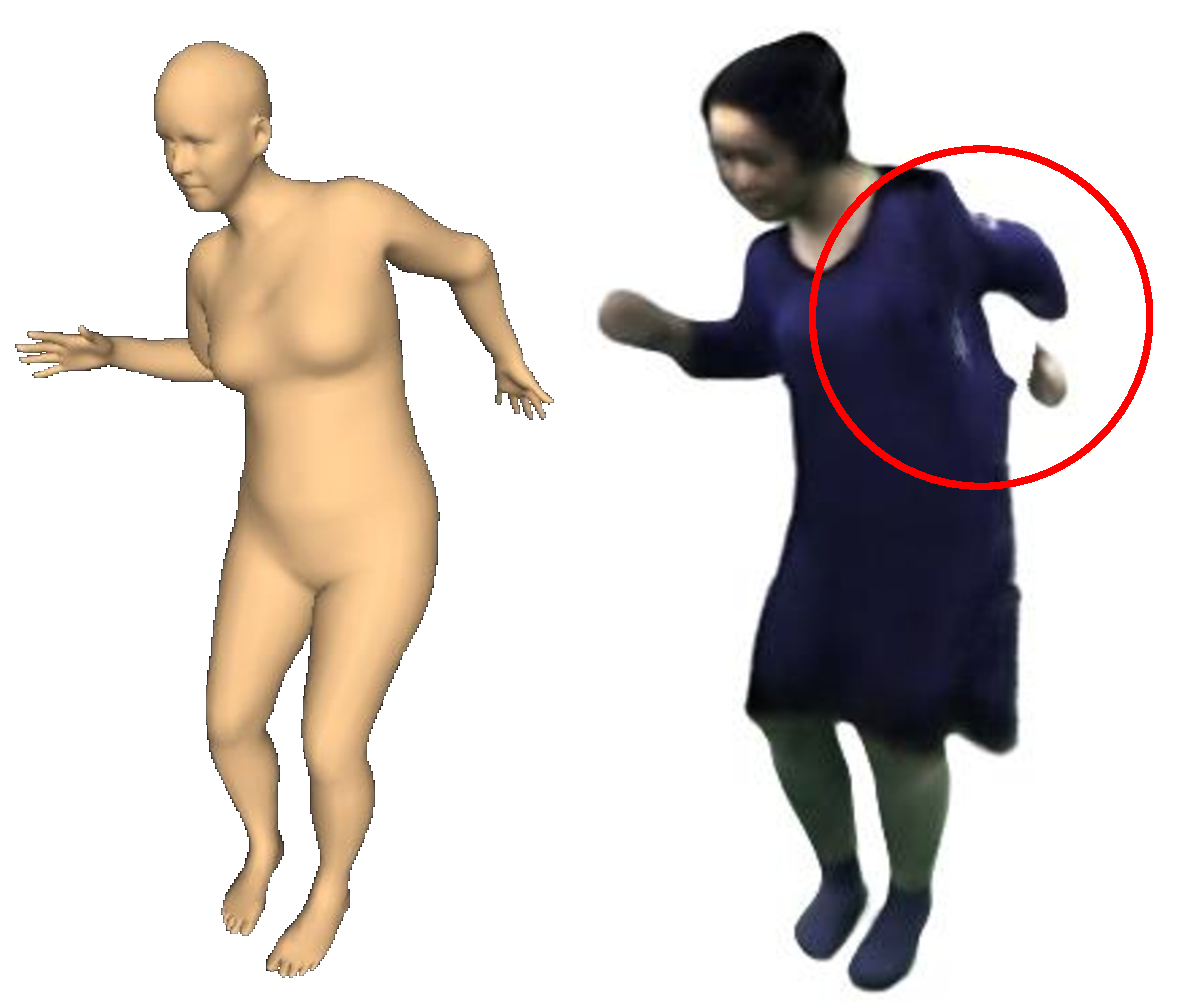
\includegraphics[width=1.01\linewidth]{failure}
%   \caption{}
% \vspace{-3mm}
\end{wrapfigure}
As we discuss in Sec.6 in the main paper, our method may fail to generate plausible results when the animation poses starkly differ from the training poses; see the inset figure on the right for an example. The main reason for this phenomenon is that neither subject-specific templates nor the SMPL surface is used to regularize shape learning in our method. 
Consequently, we cannot guarantee that our model is fully aware of the underlying geometry and its articulated surface deformation. 
Geometrical priors of clothed humans~\cite{Ma:POP:2021} can be employed to resolve this limitation and we leave it for future work. 

In addition, the dynamic deformations and wrinkle changes of garments involve complex physics processes, which may be beyond the representation capability of sparse nodes. Denser nodes could probably alleviate this limitation, but this will result in heavier computational burden. In fact, modeling the physics attributes of real-world garments is a long-standing, extremely difficult problem in computer graphics. We are currently seeking a better approach that can combine the merits of learning-based implicit representations and physics-based cloth simulation. 

